\clearpage
\section{Flow, Connectivity, and Matchings}

\subsection{Flow}

\begin{fdef}[Flow]
    Let $G$ be a directed graph with vertex set $V$ and edge set $E$. A \textit{flow} $f$ on $G$ from a vertex $s$ (the \textit{source}) to a vertex $t$ (the \textit{sink}) is a non-negative function defined on $E$ that satisfies Kirchhoff's current law: the total current flowing into each intermediate vertex (a vertex that is not the source or sink) must be equal to the total current leaving the intermediate vertex.
\end{fdef}

We usually denote $f(\vv{xy})$ by $f(x,y)$ for a flow $f$.

For any vertex $x$, define
\[
    \Gamma^+(x) = \{y\in V: \vv{xy}\in E\} \text{ and } \Gamma^-(x) = \{y\in V: \vv{yx}\in E\}
\]

Kirchhoff's current law just says that a flow $f$ from $s$ to $t$ satisfies

\[
    \sum_{y\in \Gamma^+(x)} f(x,y) = \sum_{y\in \Gamma^-(x)} f(y,x) \text{ for any }x\in V\setminus\{s,t\}.
\]

The former quantity represents the flow that exits the vertex and the latter is the flow that enters it.

Now, since the sum of flows (with direction) across all edges is $0$, we also have that

\[
    \sum_{y\in\Gamma^+(s)}f(s,y) - \sum_{y\in\Gamma^-(s)}f(y,s) = \sum_{y\in\Gamma^-(t)}f(y,t) - \sum_{y\in\Gamma^+(s)}f(t,y)
\]

This makes sense as well, since the source is the only place where flow can ``originate" and the sink is the only place it can ``terminate". This common value is known as the \textit{value} of $f$ or the \textit{amount of flow} from $s$ to $t$ and is denoted $v(f)$.\\

Obviously, there are several real problems that arise when we think of such a problem - maybe we have to transport as much water as we can from a faucet to a sink via a system of pipes. We mainly aim to \textit{maximize the flow} under some constraints.\\

\subsection{Edge Capacities -- Max-Flow and Min-Cut}

One constraint that immediately comes to mind is that each edge has a \textit{capacity} that restricts the current through the edge (the pipe can only carry so much water). That is, there is an associated non-negative number $c(x,y)$ associated with each edge $\vv{xy}$ such that any flow must satisfy $f(x,y)\leq c(x,y)$ for all edges. \\

We now introduce some additional notation to ease the process.
\begin{definition}
Given two subsets $X$ and $Y$ of $G$, we write
\[ E(X,Y)=\{\vv{xy}\in E:x\in X, y\in Y\}. \]
Whenever $g:E\to\R$ is a function, we write
\[ g(X,Y)=\sum_{\vv{xy}\in E(X,Y)} g(x,y). \]
\end{definition}

\begin{fdef}[(Edge-) Cut]
If $S$ is a subset of $V$ such that $s\in S$ but $t\not\in S$, then $E(S,\overline{S})$ is called a \textit{cut} separating $s$ from $t$ (where $\overline{S}=V\setminus S$).
\end{fdef}

The capacity of a cut $E(S,\overline{S})$ is $c(S,\overline{S})$.

Note that if we delete (the edges of) a cut from a graph, then $v(f)=0$ on the remaining graph is $0$. Indeed, there will be no path from $s$ to $t$ in this case.

Also, if there is some set of edges after whose deletion $v(f)=0$, then this set of edges must contain a cut as well.

It is also obvious that the value of any flow is at most the capacity of any cut. In particular, the maximum flow value is at most the minimum capacity of a cut.

\vspace{1mm}
We are justified in saying ``maximum" and ``minimum" here since the flow is $\leq\sum_{\vv{xy}\in E}c(x,y)<\infty$ so the set of flow values has a supremum, and there are only finitely many cuts (so they have a minimum). We encourage the reader to show that the supremum of the set of flow values is indeed attained (consider a sequence of flows such that their value converges to the supremum $v$, then the flow of each edge must converge as well).

\begin{ftheo}[Ford and Fulkerson's Max-Flow Min-Cut Theorem]
\label{maxFlow minCut}
Given a (directed) graph $G$ and a flow $f$ from $s$ to $t$, the maximum flow value from $s$ to $t$ is equal to the minimum of the capacities of cuts separating $s$ from $t$.
\end{ftheo}
\begin{proof}
Let $v$ be the maximum flow value and $f$ be the corresponding flow. Since we already know that the capacity of any cut is at least $v$, we only need to prove that a cut with such a capacity exists.  Define a subset $S\subseteq V$ as follows. To begin, $s\in S$. If $x\in S$ and
\[
    c(x,y) > f(x,y)\text{ or }f(y,x)>0
\]
then let $y\in S$. Note that if neither of the above occurs, then $f(x,y)=c(x,y)$ and $f(y,x)=0$ for every $x\in S$. We claim that $E(S,\overline{S})$ has capacity $v$.\\

First of all, we must check that $t\not\in S$. If $t\in S$, we can find vertices $s=x_0,x_1,\ldots,x_l=t$ such that
\[ \varepsilon_i = \max\{c(x_i,x_{i+1}) - f(x_i,x_{i+1}), f(x_{i+1},x_i)\} > 0 \]
for every $0\leq i<l$. Put $\varepsilon = \min_i \varepsilon_i$. Then we can construct a flow $f^*$ by increasing the flow in $\vv{x_ix_{i+1}}$ by $\varepsilon_i$ if $\varepsilon_i > f(x_{i+1},x_i)$ and decreasing the flow in $\vv{x_{i+1}x_i}$ by $\varepsilon_i$ otherwise. But if this is the case, $v(f^*) = v(f)+\varepsilon$, which contradicts the maximality of $f$.\\

Next, we must check that the capacity of this cut is indeed equal to $v$. We have
\begin{align*}
    v(f) &= \sum_{x\in S, y\in \overline{S}} f(x,y) - f(y,x) \\
    &= \sum_{x\in S, y\in \overline{S}} f(x,y) & \text{(by the construction, $f(y,x)=0$ for each such $x,y$)} \\
    &= \sum_{x\in S, y\in \overline{S}} c(x,y) = c(S,\overline{S}) & \text{(by the construction, $f(x,y)=c(x,y)$ for each such $x,y$)}
\end{align*}
Therefore, $v(f) = c(S,\overline{S})$ as desired.
\end{proof}

In the above construction, we essentially just choose those edges in the cut that are really constraining the flow from becoming any larger. All edges in the cut are such that $c(x,y)=f(x,y)$, that is, they are at maximum capacity. We add the $f(y,x) = 0$ condition to ensure that there is no ``backflow" occurring. In case we are unable to obtain such a cut, then we are able to increase the flow value along a certain trail from the source to the sink.\\
Note that this proof does not really depend on the individual capacities being finite, it merely requires that the maximum flow is finite.\\

This proof also leads to a surprisingly efficient \textit{algorithm} to find the maximal flow value if the capacity function takes only integer values.\\

Begin with a flow that is $0$ everywhere - $f_0(x,y)=0$ for all edges $\vv{xy}$. We construct an increasing (in value) sequence of flows that terminates at the maximal flow. Given $f_i$, we must find the set $S$ belonging to $f_i$ (where $S$ is that mentioned in the above proof). If $t\not\in S$, then $f_i$ is a maximal flow so we terminate. Otherwise, we can ``augment" it to a flow $f_{i+1}$ by increasing the flow along a (single) path from $s$ to $t$. \\
Since each $v(f_i)$ is an integer, we have $v(f_{i+1})\geq v(f_i)+1$ and this sequence must terminate in at most $v$ steps, where $v$ is the maximum flow value. \\

It is possible to find the set $S$ for a given flow in $\mathcal{O}(|E|)$ time, so we can find a maximal flow in $\mathcal{O}(v|E|)$ time, where $v$ is the maximum flow value.

\begin{corollary}[Integrality Theorem]
\label{integrality theorem}
If the capacity function is integral, then there is an maximal flow that is integral.
\end{corollary}

It is easy to see that this is the case from the above algorithm since the flow is integral at every step. \\

Let us now consider a seemingly more complicated situation of flow - one where there can be \textit{multiple} sources and sinks. The definition of a cut varies slightly in this case, $S$ must contain \textit{every} source and \textit{no} sink.\\
Perhaps surprisingly, this situation is no more complicated than the one we have considered so far! We can just add a single new source with an edge of infinite capacity to every source and a sink with an edge of infinite capacity from every sink. We can then extend the problem with multiple sources and sinks to one with just a single such source and sink and easily solving it as we already have.

\begin{theorem}
\label{maxFlow minCut multiple source sink}
The maximum flow value from a set of sources to a set of sinks is equal to the minimum of the capacity of cuts separating the sources from the sinks.
\end{theorem}

Let us not consider another different problem wherein we are given a function $c:V\setminus \{s,t\}\to\Rp$ such that any flow from $s$ to $t$ must satisfy
\[
\sum_{y\in\Gamma^+(x)}f(x,y) = \sum_{y\in\Gamma^-(x)}f(y,x) \leq c(x)\text{ for every }x\in V\setminus\{s,t\}
\]
That is, we are given \textit{vertex} capacities so there is a limit to the amount of water that can flow through each vertex.\\

However, this can easily be reduced to the edge capacity problem as well. Just replace each vertex $x\in V\setminus\{s,t\}$ with two vertices $x^-$ and $x^+$ such that all incoming edges to $x$ enter $x^-$, all outgoing edges exit $x^+$, and there is an edge from $x^-$ to $x^+$ of capacity $c(x)$.\\
This problem is easily seen to be equivalent to the vertex capacity problem, so we can now solve it using the Max-Flow Min-Cut Theorem.

\begin{fdef}[(Vertex-) Cut]
A \textit{cut} is a subset of $V\setminus\{s,t\}$ such that no positive-valued flow from $s$ to $t$ can be defined on $G\setminus S$.
\end{fdef}

Formulating the Max-Flow Min-Cut Theorem for vertex capacities in terms of this, we get the following theorem

\begin{theorem}
\label{maxFlow minCut vertex capacities}
Let $G$ be a (directed) graph with capacity bounds on the vertices other than the source $s$ and sink $t$. Then the minimum capacity of a vertex-cut is the maximum of the flow value from $s$ to $t$.
\end{theorem}

We can then combine \cref{maxFlow minCut}, \cref{maxFlow minCut multiple source sink}, and \cref{maxFlow minCut vertex capacities} to get

\begin{ftheo}[Generalized Max-Flow Min-Cut Theorem]
\label{generalized maxFlow minCut}

\end{ftheo}

\subsection{Menger's Theorem}

Let us now attempt to generalize the notion of connectedness of a graph slightly more.

\begin{fdef}
Let $G$ be a graph. If $G$ is connected and $G\setminus W$ is disconnected, where $W$ is either a set of vertices or edges, then $W$ is said to \textit{separate $G$}. If in $G\setminus W$, two vertices $s$ and $t$ are in different components, then $W$ is said to \textit{separate $s$ from $t$}.\\
A graph is defined to be \textit{$k$-connected} ($k\geq 2$) if it has at least $k+1$ vertices and no set of $k-1$ vertices separates it.\\
A graph is defined to be \textit{$k$-edge-connected} ($k\geq 2$) if it has at least $2$ vertices and no set of $k-1$ edges separates it.
The \textit{connectivity of a graph} $G$ is $\kappa(G)=\max_k \{G\text{ is }k\text{-connected}\}$.\\
The \textit{edge-connectivity of a graph} $G$ is $\lambda(G)=\max_k \{G\text{ is }k\text{-edge-connected}\}$.\\
\end{fdef}

If a graph $G$ is disconnected, we say that $\kappa(G)=\lambda(G)=0$.

A few points to note are:
\begin{itemize}
    \item A graph with $k+1$ vertices is $k$-connected iff it is isomorphic to $K^{k+1}$.
    \item The following are equivalent for any graph $G$ with at least $2$ vertices:
    \begin{itemize}
        \item $G$ is connected,
        \item $G$ is $1$-connected, and
        \item $G$ is $1$-edge-connected.
    \end{itemize}
    \item A graph is $2$-connected iff it is connected, has at least $3$ vertices, and has no cutvertex (Recall that a cutvertex is a vertex whose deletion increases the number of components).
    \item A graph is $2$-edge-connected iff it is connected, has at least $2$ vertices, and contains no bridge.
    \item The connectivity of a graph is the size of a smallest set of vertices that needs to be deleted to disconnect the graph. Edge connectivity is analogous.
\end{itemize}

We have the following obvious inequalities for any non-trivial graph $G$, any vertex $x\in V$, and any edge $xy\in E$:

\[\kappa(G)-1 \leq \kappa(G-x) \text{ and } \lambda(G)-1 \leq \lambda(G-xy)\leq \lambda(G) \]

\begin{theorem}[Whitney's Theorem]
For any non-trivial graph $G$, \[\kappa(G)\leq \lambda(G)\leq \delta(G).\]
\end{theorem}
\begin{proof}
The second part of this inequality is clear since deleting all the edges incident on a certain vertex (a vertex of degree $\delta(G)$ in particular) disconnects the graph.\\

For the first part, let $\lambda(G)=k$ and $S = \{x_1y_1,\ldots,x_k y_k\}$ be a set of edges whose deletion disconnects $G$.  If there is some vertex $v$ such that $v$ is not incident on any of the edges of $S$ and $C$ is the component of $G - S$ that contains $v$, then the vertices of $C$ incident on edges of $S$ (of which there are at most $k$) separates $v$ from $G\setminus C$, so $\kappa(G)\leq k$.\\[0.1cm]
Alternatively, if every vertex is incident on some edge of $S$, let $v$ be some vertex. Every neighbour $w$ of $v$ such that $v w\not\in S$ must be incident on a distinct edge of $S$ (if there were some neighbours $w_1$, $w_2$ of $v$ such that $w_1 w_2\in S$, then $S\setminus\{w_1 w_2\}$ must be disconnected as well, which contradicts the minimality of $k$. Therefore, the degree of $v$ is at most $k$. However, we also have $\delta(G)\geq k$, so the degree of every vertex ($v$ in particular) is \textit{exactly} $k$. Then, deleting the $k$ vertices adjacent to $v$ separates $v$ from the rest of the graph so $\kappa(G)\leq k$.\\
The only case where this is not valid is when $G$ has $k+1$ vertices\footnote{so when we delete the neighbours of $v$, we delete the rest of the graph}, but in this case, $G$ must be the complete graph on $k+1$ vertices(!), where we trivially have $\kappa(G)=\lambda(G)=|G|-1$.
\end{proof}

A common (incorrect) ``proof" of the above theorem just says that one can delete an arbitrary end-point of each edge to disconnect the graph, but this is not true! When we delete some vertices of the graph, we only care about connectivity among the remaining vertices! If it were indeed true, then if $\{x_1y_1,\ldots,x_k y_k\}$ was a minimal set of edges that separates the graph, then $G\setminus\{x_1,\ldots,x_k\}$ would always be disconnected. However, the following counter-example disproves the claim.

\begin{center}
    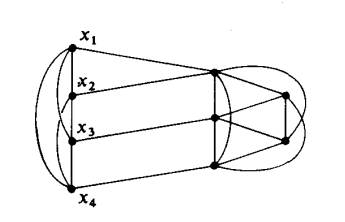
\includegraphics[scale = 0.5]{whitneyCounter.png}
\end{center}

We have already seen that it is quite useful to partition a graph into maximal connected subgraphs -- connected components (it is often be the case that proving something for a connected graph proves it for any general graph). Let us extend this to a similar partition into $2$-connected graphs.

\begin{definition}
A subgraph $B$ of a graph $G$ is a \textit{block of $G$} if either $B$ is a bridge (and its endvertices) or is a maximal $2$-connected subgraph of $G$.
\end{definition}

\begin{remark}
If $G_1$ and $G_2$ are $k$-connected subgraphs ($k\geq 1$) of a graph $G$ with at least $k$ common vertices, then $G_1\cup G_2$ is $k$-connected as well. Indeed, if we delete any $k-1$ vertices from $G_1\cup G_2$, then since what remains of $G_1$ and $G_2$ are still connected and they intersect, the entirety of the remaining graph must be connected. 
\end{remark}

Note that by the above remark, any two blocks have at most one vertex in common. Note that this also implies that distinct blocks have no edges in common.\\
If $x,y\in B$, then $G - E(B)$ contains no $x$-$y$ path (the maximality of $B$ is contradicted otherwise).\\
Therefore, a vertex is a cutvertex iff it belongs to two blocks of $G$ (Why?).

\begin{fdef}
Suppose that $G$ is a non-trivial connected graph. Define the \textit{block-cutvertex graph} $\bc(G)$ as the graph with vertices as the blocks and cutvertices of $G$ and an edge from each cutvertex to the (two) blocks containing it.
\end{fdef}

If $G$ is $2$-connected or $K^2$ (a single edge), then $\bc(G)$ is a single vertex.

We now present an important result on vertex-disjoint $s$-$t$ paths (paths from $s$ to $t$ with no common vertex).
\begin{ftheo}[Menger's Theorem]
\label{menger's theorem}
\phantom{owo}
\begin{enumerate}[(i)]
    \item Let $s$ and $t$ be distinct non-adjacent vertices of a graph $G$. Then the minimal number of vertices separating $s$ from $t$ is equal to the maximum number of independent $s$-$t$ paths.
    \item Let $s$ and $t$ be distinct vertices of $G$. Then the minimal number of edges separating $s$ from $t$ is equal to the maximum number of edge-disjoint $s$-$t$ paths.
\end{enumerate}
\end{ftheo}
\begin{proof}\phantom{owo}
\begin{enumerate}[(i)]
    \item Create a directed graph by replacing each edge $xy$ of $G$ with $\vv{xy}$ and $\vv{yx}$ and give every vertex other than $s$ and $t$ capacity $1$. By the \nameref{integrality theorem}, there is a maximal flow (from $s$ to $t$) with flow either $0$ or $1$ in each edge. Therefore, the maximum flow value is equal to the number of vertex-disjoint paths from $s$ to $t$. Now, \Cref{maxFlow minCut vertex capacities} implies that this maximum flow value is also equal to minimum capacity of a vertex-cut separating $s$ from $t$, which is just the minimal number of vertices separating $s$ from $t$ (since every vertex has capacity $1$).
    
    \item Similar to the first part, create a directed graph by replacing each edge $xy$ of $G$ with two edges $\vv{xy}$ and $\vv{yx}$ of capacity $1$ each. Using the \nameref{integrality theorem}, there is an integral maximal flow. Again, this is just equal to the edge-disjoint paths from $s$ to $t$. Using \Cref{maxFlow minCut} similar to (i) gives the result.
\end{enumerate}
\end{proof}

\begin{corollary}
A graph is $k$-connected ($k\geq 2$) iff it has at least two vertices and between any two vertices there are at least $k$ vertex-disjoint paths.\\
A graph is $k$-edge-connected ($k\geq 2$) iff it has at least two vertices and between any two vertices, there are at least $k$ edge-disjoint paths.
\end{corollary}

Note that similar to how we generalized the max-flow min-cut theorem to an arbitrary number of sources/sinks, we can similarly generalize \nameref{menger's theorem} as

\begin{theorem}[Generalized Menger's Theorem]
Let $S$ and $T$ be arbitrary subsets of vertices of $G$. Then, the maximal number of vertex-disjoint (including end-vertices\footnote{the reason for this is obvious from the construction since we add two \textit{new} vertices}) $S$-$T$ paths is equal to
\[ \min\{|W|:W\subseteq V(G), G-W\text{ has no $S$-$T$ path}\}. \]
\end{theorem}
This is easily proved by adding two new vertices $s$ and $t$, joining $s$ to every vertex in $S$, and $t$ to every vertex in $T$, and applying Menger's Theorem in the new graph.


\begin{exercise}
Let $T$ be a tree. Show that the graph whose vertices are proper $3$-colorings of $T$ and whose edges are pairs of colorings which differ at only a single vertex is connected.
\end{exercise}